% reset references counter
\setcounter{NAT@ctr}{-1}
\chapter*{}
\phantomsection\addcontentsline{toc}{section}{The Informatics: iFUSE}
\articletitle{iFUSE: integrated fusion gene explorer}
Saskia Hiltemann \textsuperscript{1}, Elizabeth A. McClellan\textsuperscript{2}, Jos van Nijnatten\textsuperscript{2}, Sebastiaan Horsman\textsuperscript{2}, Ivo Palli\textsuperscript{2}, Ines Teles Alves\textsuperscript{1,3}, Thomas Hartjes\textsuperscript{1}, Jan Trapman\textsuperscript{3}, Peter van der Spek\textsuperscript{2}, Guido Jenster\textsuperscript{1}, and Andrew Stubbs\textsuperscript{2}

\small
\begin{enumerate}
\itemsep-0.5em
\item Department of Urology, Erasmus MC, 3015 GE Rotterdam, The Netherlands.
\item Department of Bioinformatics, Erasmus MC, 3015 GE Rotterdam, The Netherlands.
\item Department of Pathology, Erasmus MC, 3015 GE Rotterdam, The Netherlands.
\end{enumerate}

Published in: Bioinformatics \\
DOI: \url{10.1093/bioinformatics/btt252} \\

\section*{Abstract}

\textbf{Summary:} We present iFUSE (integrated FUSion gene Explorer), an online visualization tool that provides a fast and informative view of structural variation data and prioritizes those breaks likely representing fusion genes. \color{black} This application uses calculated breakpoints to determine fusion genes based on the latest annotation for genomic sequence information, and where relevant the structural variation (SV) events are annotated with predicted RNA and protein sequences.\ iFUSE takes as input either a Complete Genomics (CG) junction file, a FusionMap~\cite{ge2011fusionmap} fusion detection report file, or a file already analysed and annotated by the iFUSE application on a previous occasion. \\
\textbf{Results:} We demonstrate the utility of iFUSE with case studies from tumour-normal SV detection derived from Complete Genomics whole-genome sequencing results. \\
\textbf{Availability:} iFUSE is available as a web service at \url{http://ifuse.erasmusmc.nl}


\section*{Introduction}

Structural variation analysis is a common requirement in the study of cancer where many fusion genes have been implicated in the progression of cancer~\cite{mitelman2007impact, kumar2008recurrent}
The use of next-generation sequencing for fusion gene detection in cancer~\cite{edgren2011identification, ge2011fusionmap, mcpherson2011defuse}, structural variation in non-cancerous diseases~\cite{sanders2011multiple, levy2011rare} and in normal genomes~\cite{10002010map} has expanded knowledge of the importance of these events.
In a recent study the use of \textit{de novo} assembly in association with SV detection suggests that SVs account for more diversity between individuals than do single nucleotide polymorphisms (SNPs)~\cite{li2011structural}. Complete Genomics uses \textit{de novo} assembly during SV, single nucleotide variation (SNV) and copy number variation (CNV) determination~\cite{carnevali2012computational}.

Traditionally, for a given SV, a user can visualize the individual (sides of the) breaks in viewers such as IGV~\cite{thorvaldsdottir2013integrative,robinson2011integrative}, but not the resulting event or fusion gene as a whole, and must manually retrieve the sequence of the resulting event based on the exons from both genes of the proposed fusion gene and determine the orientation and frame of the predicted transcript and encoded polypeptide sequences. Other applications also offer visualisation, but with the caveat that the user must process their data within the application, e.g inGAP-SV~\cite{qi2011ingap}, or that a bioinformatician is required to render the visualization using e.g. Circos~\cite{krzywinski2009circos}. Our aim is to deliver a web-based application that allows scientists to visualize all detected SV events and fusion genes determined in their results and to provide the concomitant candidate transcripts and polypeptide sequences associated with the detected fusion genes (\hyperref[fig:screenshot]{Figure~\ref*{fig:screenshot}}). No other application exists at the moment to categorize and visualize the candidate fusion genes, and determine the proposed sequence for gDNA, RNA and polypeptides from standard SV files.

\begin{figure}
\centerline{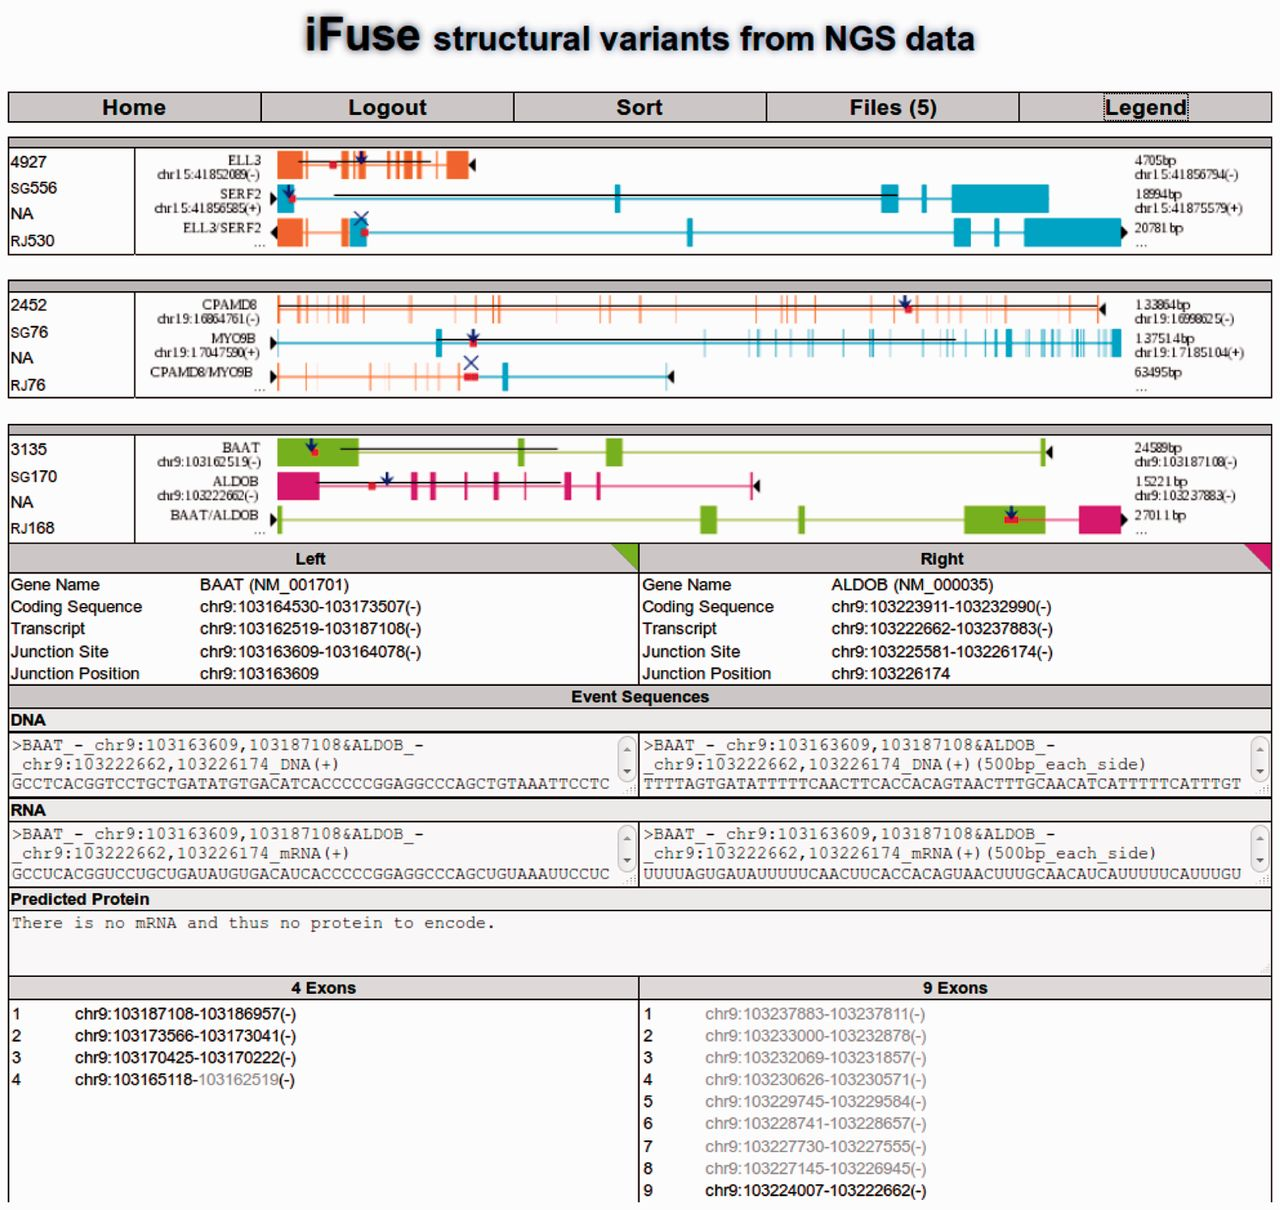
\includegraphics[width=250pt]{chapters/images/iFUSE/ifusess.jpeg}}
\caption{Screenshot of iFUSE\@. SVs are visualised and where applicable, the predicted DNA, RNA and protein sequences are reported.}
\label{fig:screenshot}
\end{figure}


\section*{Methods}

iFUSE is a PHP-coded application running on an Apache web server with a mySQL database for user management and R for data analysis. Gene-based feature annotation is provided using the UCSC gene tables (hg18 and hg19). Documentation details, including full application configuration, are available from the website (\href{http://ifuse.erasmusmc.nl}{http://ifuse.erasmusmc.nl}).

iFUSE takes as input either a Complete Genomics (CG) junctions file or a fusion detection report as generated by the FusionMap tool~\cite{ge2011fusionmap}.  To perform a comparison of two or more genomes, the Complete Genomics tool Junctions2Events can be used prior to visualisation within iFUSE\@. \color{black}
The input file is validated and then analyzed using R, after which a graphical representation for each event is generated. This representation displays the promotor, introns, exons and the junction site, and additional information including DNA, RNA and protein sequences are presented to the user. These events can be filtered and sorted by the user, either using general properties or by zooming in on a single event and filtering for nearby junctions or events with similar properties.

The input files uploaded to iFUSE are annotated in R using information retrieved from UCSC gene tables and the input files. The resulting output file can be retrieved from iFUSE for manual inspection, and can also be used directly as input to iFUSE.

Example input files can be downloaded from the downloads section of the iFUSE website and users can test the application without registration by selecting the option to start an anonymous session. Any files uploaded by the user will be deleted at the end of the anonymous session.\

iFUSE accounts are password protected, the application has been tested for security risks such as SQL injections, and our servers undergo periodical CERT vulnerability scans (http://www.cert.org). Furthermore, when a user deletes a file via the iFUSE web interface, it is purged completely from our systems.

\section*{Discussion}


Two public cancer genomes have been used to demonstrate the utility of iFUSE for the prediction of fusion genes. Genomes were downloaded from Complete Genomics (\href{ftp2.completegenomics.com}{ftp2.completegenomics.com}). The results can be found in \hyperref[tab:results]{Table~\ref*{tab:results}}.


\begin{table}[!t]
    \begin{tabular}{lcccc}
        \toprule
                              & S1 Tumour  & S1 Normal  & S2 Tumour   & S2 Normal \\
        \midrule
        HG18                  &            &            &             &         \\
        Junctions             & 1579       & 1594       & 1558        & 1387    \\
        Genes on both sides   & 32         & 15         & 23          & 4       \\
        Same orientation      & 21         & 14         & 16          & 1       \\
                              &            &            &             &         \\
        HG19                  &            &            &             &         \\
        Junctions             & 1581       & 1592       & 1559        & 1390    \\
        Genes on both sides   & 21         & 12         & 31          & 7       \\
        Same orientation      & 10         & 6          & 17          & 3       \\
        \toprule
    \end{tabular}
    \caption{Results from iFUSE on public datasets. Sample 1 (S1): HCC1187, Sample 2 (S2): HCC2218, public datasets downloadable from Complete Genomics. (ftp://ftp2.completegenomics.com/Cancer\_pairs/)
    }
    \label{tab:results}
\end{table}

An event is labeled as a fusion gene if the breakpoint has two different genes on either side. If the two sides also have the same orientation (are on the same strand, or in the case of an inversion on opposite strands) and are also in frame, the event is called a fusion protein.

\section*{Conclusion}

iFUSE provides scientists with a convenient method to visualize, categorize, and filter structural variation analysis output using Complete Genomics junction files or the FusionMap fusion detection report files as input to the application.

\section*{Acknowledgements}

This study was performed within the framework of CTMM, the Center for Translational Molecular Medicine. TraIT project (grant 05T-401).

We would like to thank Rick Tearle and Steve Lincoln from Complete Genomics whose valuable discussions on Complete Genomics analysis methods supported our application development.


\bibliographystyle{ieeetr}
\bibliography{references}
